\documentclass[10pt]{beamer}
\usepackage[italian]{babel}
\usepackage[utf8]{inputenc}

\usetheme{metropolis}
\usepackage{appendixnumberbeamer}

\usepackage{booktabs}
\usepackage[scale=2]{ccicons}

\usepackage{pgfplots}
\usepgfplotslibrary{dateplot}

\usepackage{listings}
\lstset{breaklines=true}

\usepackage{xspace}
\newcommand{\themename}{\textbf{\textsc{metropolis}}\xspace}

\title{PGP / GnuPG e reti di fiducia}
\subtitle{Un approccio distribuito alla confidenzialità, sicurezza e fiducia}
\date{28 Ottobre 2017}
\author{Enrico Bassetti}
\institute{Latina Linux User Group}
\titlegraphic{\hfill
\includegraphics[height=1.5cm]{llg.png}}

\begin{document}

\setbeamertemplate{frame footer}{Latina Linux User Group - Linux Day 2017 - PGP/GnuPG}

\maketitle

\begin{frame}{Roadmap}
  \setbeamertemplate{section in toc}[sections numbered]
  \tableofcontents[hideallsubsections]
\end{frame}

\section{Introduzione alla crittografia}

\begin{frame}[fragile]{Introduzione}

Quando Giulio Cesare comunicava con i suoi generali, come in ogni struttura
militare, voleva mantenere i messaggi segreti. Non fidandosi dei messaggeri,
iniziò quindi a scrivere i messaggi "spostando" (in inglese \textit{shift}) di 3
ogni lettera del messaggio.

In questo modo, solo chi conosceva il sistema poteva, spostando le lettere di
3 posizioni indietro, leggere il messaggio.

Questo sistema è noto come \textbf{cifrario di Cesare}.

\end{frame}

\begin{frame}[fragile]{Definizioni}
\begin{itemize}
\item \textbf{Chiave} (\textit{key}): speciale stringa segreta, utilizzata per cifrare o decifrare un messaggio (nel caso di \textit{Cesare} "3" era la \textit{chiave})
\item \textbf{Testo in chiaro} (\textit{plaintext}): il testo originale del messaggio, leggibile
\item \textbf{Cifrare} (\textit{encryption}): l'operazione che rende un testo in chiaro illegibile senza conoscere la chiave
\item \textbf{Testo cifrato}, o \textit{ciphertext}: testo "cifrato" (si presenta spesso come un "blob" di caratteri senza senso)
\item \textbf{Decifrare} (\textit{decryption}): operazione inversa della cifratura
\end{itemize}
\end{frame}

\begin{frame}[fragile]{Cifrario di Cesare: esempio}

Testo in chiaro: \textbf{ATTACCARE} \hspace{15pt} Chiave: \textbf{3}

\begin{itemize}
\item $A \rightarrow D$
\item $T \rightarrow W$
\item $T \rightarrow W$
\item $A \rightarrow D$
\item $C \rightarrow F$
\item $C \rightarrow F$
\item $A \rightarrow D$
\item $R \rightarrow U$
\item $E \rightarrow H$
\end{itemize}

Testo cifrato: \textbf{DWWDFFDUH}

\end{frame}
\begin{frame}[fragile]{Problemi con il cifrario di Cesare}

\textbf{ATTACCARE}

\textbf{DWWDFFDUH}

Vedete qualche problema con il cifrario?

\begin{itemize}
\item \pause Le stesse lettere sono codificate allo stesso modo - in altre parole, se una lettera si ripete nel messaggio "in chiaro", allora si ripete anche nel messaggio cifrato.
\item \pause Semplicemente provando tutte le 25 possibili combinazioni (35 se si considerano i numeri), si può risalire al numero di spostamenti necessari!!
\end{itemize}

\end{frame}

\begin{frame}[fragile]{Sistemi di crittografia moderni}

Esistono sistemi più efficaci per generare "testo cifrato" dal testo non cifrato usando una chiave. I più importanti sono:

\begin{itemize}
\item AES
\item RSA
\item ElGamal
\end{itemize}

Tutti si basano sulla difficoltà di risolvere problemi matematici, ad esempio il \textit{logaritmo discreto} o la \textit{fattorizzazione in numeri primi}.

\end{frame}

\begin{frame}[fragile]{La crittografia nella vita quotidiana}

Molti sistemi che utilizziamo abitualmente usano un sistema crittografico. Ad esempio:

\begin{itemize}
\item La rete GSM/UMTS (chiamate voce e SMS)
\item Siti internet HTTPS (la banca, PayPal, Amazon, etc)
\item Tutti i sistemi di posta elettronica forniscono l'accesso anche in modo sicuro con SSL
\item ...
\end{itemize}

\end{frame}

\section{Sistemi a chiave simmetrica e asimmetrica}

\begin{frame}[fragile]{Definizioni}

Per sistema a \textbf{chiave simmetrica} si intende un sistema di trasmissione che utilizza la stessa chiave per \textit{cifrare} e \textit{decifrare} il messaggio. Il cifrario di Cesare è un sistema a chiave simmetrica.

Un sistema che impiega due chiavi diverse per la crittazione e la decrittazione è detto a \textbf{chiave asimmetrica}. In genere si utilizza il termine \textbf{chiave pubblica} per la chiave di crittazione, e \textbf{chiave privata} per la chiave di decrittazione.

\end{frame}

\begin{frame}{Chiave simmetrica}

Un sistema di crittazione con chiave simmetrica si basa sulla presenza di un \textbf{segreto condiviso}, ovvero della chiave.

Questa chiave deve essere \textbf{già} condivisa tra i due (o più) soggetti della comunicazione in modo sicuro.

\centering
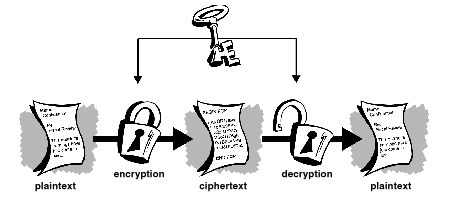
\includegraphics[scale=0.5]{symmetric-cryptography}

\end{frame}

\begin{frame}{Chiave asimmetrica}

La chiave \textbf{pubblica} è una chiave che può essere utilizzata per crittografare un messaggio, ma non può essere utilizzata per l'operazione inversa. In altre parole, una volta crittato un file con la chiave pubblica, non è possibile leggerlo se non utilizzando la chiave \textbf{privata}.

Questa operazione permette l'invio di messaggi tra due soggetti senza che venga condiviso un segreto.

\centering
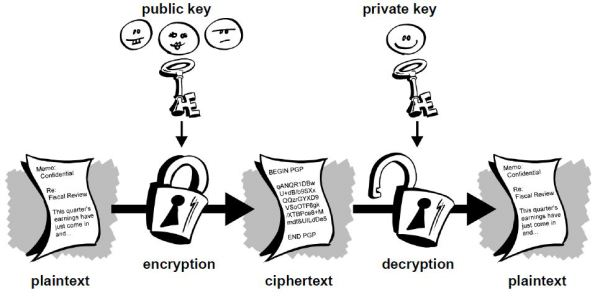
\includegraphics[scale=0.4]{public-key-cryptography}

\end{frame}

\section{Verificare l'integrità con la crittografia}

\begin{frame}{Integrità del messaggio}

In taluni casi è necessario verificare l'integrità del messaggio, ovvero verificare che non sia stato alterato (pensiamo ad un codice IBAN per un versamento).

Esistono algoritmi che generano un codice di verifica (chiamato \textbf{hash}) con il quale si può verificare che il testo non sia stato alterato. Ma come possiamo essere sicuri che anche questo codice non venga alterato?

\end{frame}

\begin{frame}{Integrità del messaggio (2)}

Usando un sistema crittografico (con chiave simmetrica o asimmetrica) possiamo crittografare il messaggio (o il codice di verifica): in questo modo il messaggio diventa inalterabile a meno di conoscere le chiavi.

Nel caso si usi un sistema a chiave \textbf{simmetrica}, è sufficiente crittare l'\textit{hash} generato con la chiave e allegarlo al messaggio: solo il destinatario potra aprire, conoscendo la chiave, l'hash generato e verificare che il messaggio non è stato alterato.

Nel caso si usi un sistema a chiave \textbf{asimmetrica}, si invertono i ruoli delle chiavi \textbf{pubblica} e \textbf{privata}: la prima viene usata per decrittografare l'\textit{hash} (in fase di verifica), mentre la seconda per \textbf{crittografare} l'\textit{hash} (in fase di firma).

\end{frame}

\section{La Fiducia in un sistema asimmetrico}

\begin{frame}{Vi presento Alice, Bob e Trudy}

Immaginiamo che \textit{Alice} debba inviare a \textit{Bob} un file importante, e di volerlo crittografare con una coppia di chiavi asimmetriche per evitare che \textit{Trudy} possa leggerlo.

Per farlo, \textit{Alice} userà la sua \textbf{chiave pubblica}, così che \textbf{solo} \textit{Bob} possa, con la sua \textbf{chiave privata}, leggere il contenuto del file.

Ma come possiamo avere la chiave pubblica di Alice in modo sicuro?

\centering
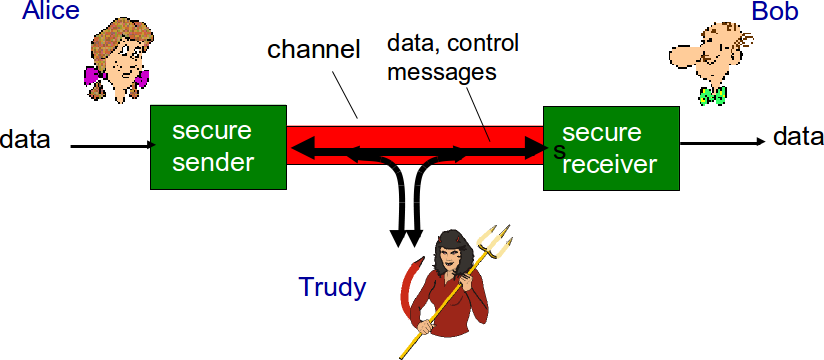
\includegraphics[scale=0.4]{1-alice-bob-trudy}

\end{frame}

\begin{frame}{La chiave di Alice}

\textit{Bob}, per ottenere la chiave pubblica di \textit{Alice}, può:

\begin{itemize}
\item Scaricarla da internet o farsela inviare via e-mail: in questo modo però \textit{Trudy} potrebbe intercettare la comunicazione e scambiare la chiave pubblica di \textit{Alice} con la sua; così \textit{Bob} crittografa il file con la chiave di \textit{Trudy} anziché di \textit{Alice}, e quindi \textit{Trudy} può leggere il contenuto
\item Usare un server esterno: e se \textit{Trudy} controllasse quel server?
\item Incontrare \textit{Alice} di persona: il metodo è sicuro, ma non sempre è fattibile
\item Fidarsi di \textit{Charlie} (del quale anche \textit{Alice} si fida), per scambiare la chiave
\end{itemize}

Ogni sistema ha le sue falle e le sue peculiarità. In generale due approcci sono usati per risolvere questo problema: \textbf{PKI} e \textbf{Web-of-trust}

\end{frame}

\begin{frame}{PKI e web-of-trust}

\begin{itemize}
\item \textbf{Public Key Infrastructure}: la fiducia in una chiave (e le informazioni in essa contenute) si basa sulla fiducia in un terzo (rispetto ad \textit{Alice} e \textit{Bob}) che garantisce per entrambi
\item \textbf{Web-of-trust}: la fiducia in una chiave si basa su una rete di persone fidate tra \textit{Alice} e \textit{Bob}
\end{itemize}

\end{frame}

\begin{frame}{PKI e web-of-trust}

\includegraphics[scale=0.15]{pgp_vs_ca}

\end{frame}

\begin{frame}{Public Key Infrastructure}

Nella \textit{Public Key Infrastructure} vengono generate delle coppie di chiavi pubblica-privata per un ente detto \textit{Certification Authority}. Dopodiché la \textit{CA} fornisce a tutti una copia della sua chiave pubblica (in modo "sicuro") e firma (con un procedimento che vedremo dopo) le chiavi delle persone di cui si fida.

In questo modo si crea una catena di certificati (detta \textit{certificate chain}) che portano da \textit{Alice} alla \textit{CA}. \textit{Bob}, fidandosi della \textit{CA}, si fida anche della chiave di \textit{Alice} firmata dalla \textit{CA}

\end{frame}

\begin{frame}{Public Key Infrastructure (2)}

Le chiavi delle \textit{autorità di certificazione} vengono inserite in modo predefinito all'interno del sistema operativo, anche se le applicazioni possono avere una loro lista "personale" (ad esempio i browser). \textbf{Installare nel proprio computer un certificato CA equivale quindi a fidarsi di tutti i certificati emessi da quella CA}

In generale, sono inserite come \textit{CA} enti importanti come:
\begin{itemize}
\item Verisign
\item Microsoft
\item Thawte
\item GlobalSign
\item ...
\end{itemize}

\end{frame}

\begin{frame}{Web-of-trust}

Usando un sistema di \textbf{web-of-trust} invece si crea una rete di persone che firmano e danno "fiducia" alle chiavi di altre persone. In particolare, ci sono due operazioni:

\begin{itemize}
\item \textbf{Firma della chiave} di una persona (di un conoscente) dopo che si è verificato che la persona sia veramente lui (ad esempio, se \textit{Bob} è cresciuto insieme a \textit{Charlie}, allora, dopo aver ottenuto a mano la chiave da \textit{Charlie}, la firmerà così da confermare che la chiave è associata a lui)
\item \textbf{Fiducia in una chiave}: si può impostare una fiducia (di default è nulla) su di una chiave, in base a quanto ci si fida della persona: questo cambia il modo in cui si considerano le chiavi firmate da quella persona (esempio \textit{Bob} si fida completamente di \textit{Charlie}, quindi \textbf{ha fiducia nel fatto che \textit{Charlie} verifichi le chiavi che firma})
\end{itemize}

\end{frame}

\section{PGP/GPG e Web-of-trust}

\begin{frame}{PGP/GnuPG}

\textbf{PGP}, acronimo di \textit{Pretty Good Privacy} è un software scritto da \textit{Phil Zimmermann} nel 1991 come sistema di crittografia a chiavi asimmetriche. Dal suo software sono derivati i prodotti commerciali \textbf{PGP Corp} (attualmente di \textit{Symantec}) e lo standard libero \textbf{OpenPGP}.

\textbf{GnuPG} (GPG) è una implementazione libera (con licenza GPL) dello standard OpenPGP, fa parte dei progetti \textit{GNU}. GPG è un software a riga di comando, ma esistono interfacce grafiche per facilitare l'utilizzo.

\end{frame}

\begin{frame}{GPG e la fiducia}

I livelli di fiducia a disposizione con PGP/GPG sono:

\begin{itemize}
\item \textbf{Sconosciuta}: nessun valore di fiducia associato (di default quando importiamo le chiavi dentro il nostro archivio locale)
\item \textbf{Nessuna}: nessuna fiducia, la persona firma chiavi impropriamente (eg. senza verificarne il proprietario)
\item \textbf{Marginale/parziale}: sappiamo che la persona comprende le implicazioni del sistema e firma propriamente le chiavi
\item \textbf{Completa}: la persona conosce a fondo il sistema e possiamo fidarci completamente
\end{itemize}

\end{frame}

\begin{frame}{GPG e la rete di fiducia}

I livelli di fiducia sono utilizzati per determinare se una chiave è affidabile, per transitività. Per far questo, GPG considera una chiave \textbf{K} valida se:

\begin{itemize}
\item \textbf{K} è firmata da un numero sufficiente di chiavi valide, ovvero:
\begin{itemize}
\item \textbf{K} è firmata personalmente da te
\item \textbf{K} è firmata da una delle chiavi che ritieni \textbf{completamente} affidabili
\item \textbf{K} è firmata da almeno 3 chiavi \textbf{parzialmente} affidabili
\end{itemize}
\item il percorso tra la tua chiave e \textbf{K} è al massimo di 5 passi (5 chiavi)
\end{itemize}

I numeri qui esposti sono i valori di default di GPG, ma possono essere modificati a piacimento

\end{frame}

\begin{frame}{GPG e la rete di fiducia}

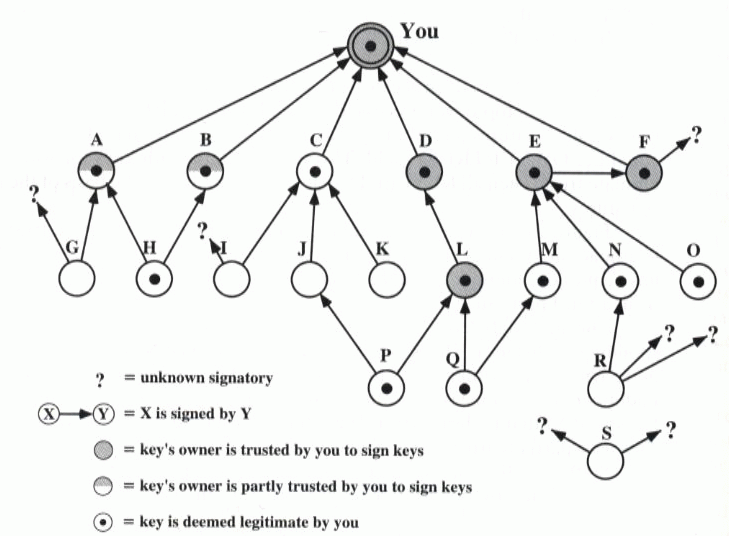
\includegraphics[scale=0.4]{pgp_web}

\end{frame}

\section{Hands-on: Usare GPG}

\begin{frame}[fragile]{PRE: impostazioni consigliate}

Configurazione consigliata per `~/.gnupg/gpg.conf`:

\begin{lstlisting}
personal-digest-preferences SHA256
cert-digest-algo SHA256
default-preference-list SHA512 SHA384 SHA256 SHA224 AES256 AES192 AES CAST5 ZLIB BZIP2 ZIP Uncompressed
\end{lstlisting}

PS: da `default-preference-list` a `Uncompressed` è solo una riga

\end{frame}

\begin{frame}[fragile]{Generare una chiave con GPG}

\begin{verbatim}
$ gpg --gen-key
\end{verbatim}

I passi (guidati) per la creazione sono:

\begin{enumerate}

\item Scelta degli algoritmi, tra DSA+RSA, DSA+ElGamal, DSA (solo firma) o RSA (solo firma)
\item Scelta della lunghezza della chiave (in bit)
\item Scelta della data di scadenza
\item Specifica dello user-id (nome, e-mail ed eventuale commento)
\item Password di protezione per la chiave privata

\end{enumerate}

A questo punto vengono stampate diverse informazioni riguardo alla chiave: le più importanti sono l'e-mail dello user-id e l'ID della chiave.

\end{frame}

\begin{frame}[fragile]{Lista delle chiavi sul PC}

Possiamo visualizzare la lista delle chiavi pubbliche presenti sul nostro PC con il comando:

\begin{verbatim}
$ gpg --list-keys
\end{verbatim}

Mentre per le chiavi private:

\begin{verbatim}
$ gpg --list-secret-keys
\end{verbatim}

\end{frame}

\begin{frame}[fragile]{Crittografare un file: per noi}

\begin{verbatim}
$ gpg --encrypt --recipient nostro@user.id nomefile.ext
\end{verbatim}

Il sistema provvederà a crittografare il file (salvandolo come `nomefile.ext.gpg`) con la chiave pubblica dello user-id indicato (in questo caso il nostro)

Per decrittografarlo, dobbiamo avere la chiave privata sul PC e dobbiamo digitare:

\begin{verbatim}
$ gpg nomefile.ext.gpg
\end{verbatim}

GPG ci chiederà la password per sbloccare la chiave privata, e creerà il file `nomefile.ext` con il plaintext.

\end{frame}

\begin{frame}[fragile]{Crittografare un file: per qualcun altro}

Immaginando che Bob abbia, come e-mail nello user-id della chiave, `amico@user.id`:

\begin{verbatim}
$ gpg --encrypt --recipient amico@user.id nomefile.ext
\end{verbatim}

Il sistema provvederà a crittografare il file (salvandolo come `nomefile.ext.gpg`) con la chiave pubblica dello user-id indicato (in questo caso, \textbf{`amico@user.id`}).

Fatto questo, non possiamo leggere il file `*.gpg`: per farlo ci serve la chiave privata di Bob, \textbf{che non abbiamo}! Solo lui potrà decrittografarlo con il comando visto nella precedente slide.

\end{frame}

\begin{frame}[fragile]{Integrità: firmare un file}

E' possibile firmare un file in modo "autocontenuto", ovvero salvando firma e file originale all'interno di un solo file:

\begin{verbatim}
$ gpg --sign --recipient nostro@user.id file.txt
\end{verbatim}

Il sistema provvederà a firmare il file (salvandolo come `nomefile.ext.gpg`) con la chiave privata del nostro user-id.

Se si vuole lasciare separato il file originale (ad esempio per file di grandi dimensioni può esser comodo):

\begin{verbatim}
$ gpg --armor --detach-sig --recipient nostro@user.id file.txt
\end{verbatim}

In questo caso il file `*.gpg` conterrà \textbf{solo} la firma.

\end{frame}

\begin{frame}[fragile]{Integrità: verificare una firma}

Per verificare la firma di un file autocontenuto (firma+originale):

\begin{verbatim}
$ gpg --verify file.txt.gpg
\end{verbatim}

Mentre, per estrarre il file originale:

\begin{verbatim}
$ gpg --output file.txt --decrypt file.txt.gpg
\end{verbatim}

Altrimenti, se si sono separati firma e file originale, è possibile verificare la firma con:

\begin{verbatim}
$ gpg --verify file.txt.gpg file.txt
\end{verbatim}

\end{frame}

\begin{frame}[fragile]{Revocare una chiave}

Se la chiave è stata compromessa, o se la si vuole per qualche motivo dismettere (cessato utilizzo, etc), bisogna dapprima generare la revoca:

\begin{verbatim}
$ gpg --armor --output revoke.asc --gen-revoke KEYID
\end{verbatim}

E poi importare il file di revoca:

\begin{verbatim}
$ gpg --import revoke.asc
\end{verbatim}

\textbf{Questa azione è irreversibile}.

E' possibile comunque continuare a decrittografare i file e verificare le firme, ma non è più possibile generare firme valide o crittografare nuovi file.

\end{frame}

\begin{frame}[fragile]{Web-of-trust: i keyserver}

Per comodità, le chiavi pubbliche possono essere inviate/ricevute a/da "keyserver", ovvero server appositamente creati per ospitare chiavi. Per pubblicare (o aggiornare) la nostra chiave:

\begin{verbatim}
$ gpg --keyserver pgp.mit.edu --send-key IDCHIAVE
\end{verbatim}

Per scaricare la chiave di qualcuno:

\begin{verbatim}
$ gpg --keyserver pgp.mit.edu --recv-key IDCHIAVE
\end{verbatim}

I server più comuni sono `pgp.mit.edu` e `pool.sks-keyservers.net`.

\end{frame}

\begin{frame}[fragile]{Web-of-trust: firmare le chiavi di altre persone}

\begin{verbatim}
$ gpg --recipient nostro@user.id --sign-key KEYID
\end{verbatim}

Dopo averle firmate, è conveniente re-inviare la chiave sui keyserver, in modo che la firma sia visibile a tutti.

\end{frame}

\begin{frame}[fragile]{Email e GPG}

E' possibile firmare (e/o crittografare) le e-mail in uscita e verificare la firma (e/o decrittografare) le e-mail in entrata nei vari client di posta elettronica tramite plugins.

\begin{itemize}
\item Thunderbird: Enigmail
\item MS Outlook: Gpg4win
\item Apple Mail.app (macOS): GPGMail
\end{itemize}

\end{frame}

\begin{frame}[standout]
  Questions?
\end{frame}

\begin{frame}{Conclusioni}

  \begin{center}\ccbysa\end{center}
  
  \centering https://github.com/Enrico204/ld2017-gpg

\end{frame}

\end{document}
